% Báo cáo riêng; không sửa bao_cao_tien_do.tex.
% Biên dịch từ baocao1: xelatex bao_cao_benchmark.tex (hai lần).
% Hoặc: tectonic bao_cao_benchmark.tex --keep-logs
% Ảnh dùng đường dẫn tương đối, nằm hoàn toàn trong baocao1/figures/.
\documentclass[11pt,a4paper]{article}
\usepackage{fontspec}
\IfFontExistsTF{TeX Gyre Termes}{\setmainfont{TeX Gyre Termes}}{\setmainfont{DejaVu Serif}}
\IfFontExistsTF{TeX Gyre Heros}{\setsansfont{TeX Gyre Heros}}{\setsansfont{DejaVu Sans}}
\IfFontExistsTF{Latin Modern Mono}{\setmonofont{Latin Modern Mono}}{\setmonofont{DejaVu Sans Mono}}
\usepackage[vietnamese]{babel}
\usepackage[left=2.4cm,right=2.2cm,top=2.2cm,bottom=2.2cm]{geometry}
\usepackage{amsmath,amssymb,booktabs,tabularx,array}
\usepackage{graphicx,float,pdflscape,caption,enumitem,setspace}
\usepackage[table]{xcolor}
\usepackage[unicode,colorlinks=true,linkcolor=blue!45!black,citecolor=blue!45!black,urlcolor=blue!45!black]{hyperref}
\usepackage{xurl}
\setstretch{1.06}
\setlength{\parindent}{1.2em}
\setlength{\parskip}{0.25em}
\setlength{\emergencystretch}{3em}
\renewcommand{\arraystretch}{1.18}
\setlist{itemsep=0.2em,topsep=0.3em,leftmargin=*}
\captionsetup{font=small,labelfont=bf}
\newcolumntype{Y}{>{\raggedright\arraybackslash}X}
\newcolumntype{P}[1]{>{\raggedright\arraybackslash}p{#1}}
\newcommand{\NA}{\textemdash}
\newcommand{\pct}[1]{#1\%}
\newcommand{\code}[1]{\begingroup\small\urlstyle{same}\path{#1}\endgroup}
\definecolor{paperrose}{RGB}{252,231,230}
\definecolor{papercyan}{RGB}{228,246,250}
\definecolor{projectgreen}{RGB}{229,243,233}
\title{\textbf{BÁO CÁO KẾT QUẢ BENCHMARK}\\[0.5em]
\large P-CRA-U: grounding công khai, nguyên nhân giới hạn chuyển miền\\
và hướng cải tiến kiến trúc}
\author{Đồ án: Nghiên cứu phương pháp suy luận không gian và hiệu chuẩn\\
độ bất định cho Spatial Vision--Language Model trong thao tác robot}
\date{Ngày 7 tháng 10 năm 2026}

\begin{document}
\begin{center}
{\Large\bfseries BÁO CÁO KẾT QUẢ BENCHMARK\par}
\vspace{0.35em}
{\normalsize P-CRA-U: grounding công khai, nguyên nhân giới hạn chuyển miền\par
và hướng cải tiến kiến trúc\par}
\vspace{0.5em}
{\small Đồ án: Nghiên cứu phương pháp suy luận không gian và hiệu chuẩn\par
độ bất định cho Spatial Vision--Language Model trong thao tác robot\par}
\vspace{0.4em}
{\small Ngày 7 tháng 10 năm 2026\par}
\end{center}
\begin{abstract}
Báo cáo tổng hợp RefSpatial-Bench Location và hai pilot RefCOCO/RefCOCO+ val,
mỗi pilot 100 ảnh/300 câu. Grounding Sidecar đạt \pct{33,67}/\pct{30,67};
grounding RoboRefer RGB-D đạt \pct{93,67}/\pct{91,00}. Hướng hiện hành giữ
điểm RoboRefer, bổ sung anchor và kiểm chứng quan hệ, rồi hiệu chuẩn lại cho
prediction mới. Nhánh primary đã chạy inference; calibration chưa hoàn tất.
\end{abstract}

\section{Phạm vi đánh giá và quy ước}
\subsection{Hai biến thể P-CRA-U được phân biệt}
\textbf{P-CRA-U--Sidecar (Tasks60 MC):} điểm cuối là MAP của target head học
riêng từ features RoboRefer và text encoder riêng.

\textbf{P-CRA-U--RoboRefer primary (hướng hiện tại):} điểm cuối do VLM đầy đủ
sinh; Sidecar bổ sung anchor/diagnostics. Grounding được kế thừa từ backbone,
chưa là cải thiện RoboRefer do verifier hoặc uncertainty.

\subsection{Các tập đã chạy và metric}
\begin{table}[H]\centering\small
\caption{Phạm vi thực nghiệm. Đơn vị chấm là câu lệnh, không phải chỉ số ảnh.}
\begin{tabularx}{\linewidth}{P{3.7cm} P{3.4cm} Y}
\toprule
Benchmark & Phạm vi đã chạy & Điều kiện điểm đúng\\
\midrule
RefSpatial-Bench Location & 100 câu; 61 RGB SHA256 khác nhau & Điểm nằm trong mask target\\
RefCOCO UNC val & Pilot 100 ảnh, 300 câu, 202 references & Điểm nằm trong GT bbox\\
RefCOCO+ UNC val & Pilot 100 ảnh, 300 câu, 194 references & Điểm nằm trong GT bbox\\
\bottomrule
\end{tabularx}
\end{table}

Point-in-box là cách chấm point dùng trong phần referring 2D của RoboRefer
\cite{roborefer}; nó khác IoU của một bbox dự đoán và khác point-in-mask.
Với hộp GT $B_i=(x_i,y_i,w_i,h_i)$, điểm $\hat p_i=(\hat x_i,\hat y_i)$ được
chấm bằng $\mathbf{1}[\hat p_i\in B_i]$, đồng thời phải nằm trong ảnh.
Không so trực tiếp \pct{6,00} point-in-mask với \pct{33,67} point-in-box như
một mức cải thiện trên cùng event.

\begin{landscape}
\section{Bảng đối chiếu với các mô hình trong bài báo RoboRefer}
\begin{table}[H]\centering
\caption{Các hàng tham khảo được dựng lại từ Table 3 của RoboRefer
\cite{roborefer}; các hàng đồ án được thêm ở cuối. Giá trị là phần trăm.
Hàng pilot chỉ điền vị trí val, các split chưa chạy ghi \NA.}
\label{tab:paper-comparison}
\begingroup\small
\setlength{\tabcolsep}{4pt}
\renewcommand{\arraystretch}{1.24}
\begin{tabular}{P{6.0cm} c c c c P{2.6cm}}
\toprule
Phương pháp & Output & RefCOCO & RefCOCO+ & RefCOCOg & Phạm vi\\
 & & val / testA / testB & val / testA / testB & val / test & số liệu\\
\midrule
\rowcolor{paperrose}\multicolumn{6}{c}{\textit{Grounding Specialist Models -- số công bố trong paper}}\\
GroundingDINO & BBox & 90.6 / 93.2 / 88.2 & 88.2 / 89.0 / 75.9 & 86.1 / 87.0 & Theo paper\\
\rowcolor{paperrose}\multicolumn{6}{c}{\textit{Open-Source Vision-Language Models -- số công bố trong paper}}\\
Qwen2.5-VL-72B & BBox & 92.7 / 94.6 / 89.7 & 88.9 / 92.2 / 83.7 & 89.9 / 90.3 & Theo paper\\
Qwen2.5-VL-72B & Point & 95.2 / 96.5 / 93.8 & 90.4 / 93.5 / 86.7 & 91.5 / 92.0 & Theo paper\\
Qwen2.5-VL-72B & B.$\to$P. & 95.4 / 97.0 / 94.2 & 91.5 / 94.9 / 88.2 & 92.5 / 92.5 & Theo paper\\
\rowcolor{papercyan}\multicolumn{6}{c}{\textit{RoboRefer Variants -- số công bố trong paper}}\\
RoboRefer-2B-SFT & Point & 95.5 / 96.7 / 93.8 & 91.8 / 94.3 / 86.3 & 93.3 / 93.6 & Theo paper\\
RoboRefer-8B-SFT & Point & 96.6 / 97.7 / 94.7 & 91.9 / 95.2 / 87.5 & 94.3 / 94.1 & Theo paper\\
RoboRefer-2B-RFT & Point & 95.6 / 96.6 / 93.9 & 92.0 / 94.2 / 86.3 & 93.2 / 93.63 & Theo paper\\
\rowcolor{projectgreen}\multicolumn{6}{c}{\textit{Đồ án -- pilot val 100 ảnh / 300 câu cho mỗi benchmark}}\\
P-CRA-U--Sidecar, Tasks60 MC & Point & 33.67 / \NA{} / \NA & 30.67 / \NA{} / \NA & \NA{} / \NA & Pilot val\\
\textbf{P-CRA-U--RoboRefer primary} & Point & \textbf{93.67} / \NA{} / \NA & \textbf{91.00} / \NA{} / \NA & \NA{} / \NA & \textbf{Pilot val}\\
RoboRefer RGB-only, ảnh gốc (đối chứng) & Point & 92.33 / \NA{} / \NA & 88.33 / \NA{} / \NA & \NA{} / \NA & Pilot val\\
\bottomrule
\end{tabular}
\endgroup
\end{table}

\noindent\footnotesize
\textbf{Cách đọc bảng.} BBox, Point và B.$\to$P. giữ cách ghi của paper;
B.$\to$P. là chuyển bbox dự đoán thành điểm ở tâm hộp. Các số BBox được giữ
nguyên từ nguồn, không chấm lại bằng evaluator point của đồ án.
Các hàng paper theo split công bố, còn đồ án là subset pilot;
\textbf{không xếp hạng SOTA từ các hàng này}.
Không điền số pilot vào các cột testA, testB hoặc RefCOCOg chưa đánh giá.

\smallskip
\noindent\textbf{Điều kiện chạy của đồ án.} Primary dùng RoboRefer-2B-SFT
RGB-D $640\times480$ và greedy decoding. Đối chứng RGB-only dùng ảnh gốc.
Chưa tái hiện chính xác toàn bộ thiết lập/split của paper. Hai pilot có 96 ảnh
trùng image ID nhưng khác câu/target; không xem chúng là 200 cảnh độc lập.

\smallskip
\noindent\textbf{Trạng thái phương pháp.} Primary giữ nguyên điểm backbone,
không chọn giữa hai điểm bằng nhãn thật. Điểm cao hơn Sidecar cho thấy lợi ích
của việc giữ đường grounding VLM đầy đủ; chưa chứng minh Sidecar, verifier hoặc
MC Dropout làm backbone dự đoán tốt hơn. Risk và threshold của primary hiện
chưa được hiệu chuẩn.
\end{landscape}

\section{Kết quả thực nghiệm đã chạy}
\subsection{Protocol của hai pilot referring 2D}
Nguồn dữ liệu là mirror \texttt{jxu124/refcoco-benchmark} \cite{refer} với revision cố định
\code{2f2f892835bbf44b4db81f1c4ad6d46a3e9e4359}. Hai parquet val đã được
kiểm tra SHA256 theo LFS. RefCOCO val đầy đủ có 1.500 ảnh/10.834 câu;
RefCOCO+ val có 1.500 ảnh/10.758 câu. Mỗi pilot chỉ chọn 100 ảnh có ít nhất
3 câu và 3 câu mỗi ảnh bằng thứ hạng SHA256, seed 24082026, trước forward.
Không lọc mẫu theo độ chính xác mô hình. Raw phrase được giữ nguyên, chỉ thêm
cấu trúc lệnh \texttt{Locate} và suffix định dạng điểm cho RoboRefer.

Depth Anything V2 Large suy pseudo-depth từ RGB gốc, min--max thành ảnh uint8
ba kênh rồi resize bilinear cùng RGB về $640\times480$. Đây là relative depth
làm input, không phải GT depth theo mét. RoboRefer sinh greedy với tối đa
128 tokens. Sidecar dùng cùng visual features; MC chạy 20 passes ở nhánh phụ trợ.
Masks/bboxes và nhãn chỉ vào evaluator sau khi lưu predictions.

\begin{table}[H]\centering\small
\caption{Kết quả theo đúng các pilot đã chạy. CI95 được bootstrap 10.000 lượt
theo nhóm image ID, 100 nhóm/pilot.}
\label{tab:pilot-results}
\begin{tabularx}{\linewidth}{P{3.0cm} Y c c}
\toprule
Benchmark & Nguồn target & Đúng / tổng & Accuracy [CI95]\\
\midrule
RefCOCO & Sidecar Tasks60 & 101/300 & 33,67 [27,67;39,67]\\
 & RoboRefer primary & 281/300 & 93,67 [91,00;96,33]\\
 & RoboRefer RGB-only gốc & 277/300 & 92,33\\
\midrule
RefCOCO+ & Sidecar Tasks60 & 92/300 & 30,67 [25,00;36,67]\\
 & RoboRefer primary & 273/300 & 91,00 [87,33;94,33]\\
 & RoboRefer RGB-only gốc & 265/300 & 88,33 [83,67;92,67]\\
\bottomrule
\end{tabularx}
\end{table}

Trên RefCOCO, đổi nguồn target sang RoboRefer sửa 187 câu và làm sai 7 câu
so với Sidecar; delta $+60,00$ điểm phần trăm (pp), CI95 $[53,33;66,33]$ pp.
Trên RefCOCO+, sửa 187 và làm sai 6 câu; delta $+60,33$ pp,
CI95 $[54,00;66,67]$ pp. Không chọn nhánh theo GT từng câu.
RefCOCO là replay predictions đã lưu sau khi quan sát pilot cũ, kèm một case
đã chạy live lại; RefCOCO+ có 300 generations RGB-D mới và 300 generations
RGB-only đối chứng. Tọa độ primary khớp parser điểm official 300/300 ở mỗi pilot.

RefCOCO+ có 27 lỗi trên 23 ảnh; 77/100 ảnh đúng cả ba câu và 99/100 ảnh đúng
ít nhất một câu. Hai lỗi cách bbox không quá 2 pixel ảnh gốc vẫn được giữ là
lỗi trong metric chính. Primary RGB-D hơn RGB-only gốc $2,67$ pp, CI95
$[0,00;5,33]$ pp; hai nhánh khác cả độ phân giải/preprocessing và depth,
nên không quy riêng chênh lệch cho depth.

\subsection{RefSpatial-Bench Location: kết quả khó hơn về spatial referring}
\begin{table}[H]\centering\small
\caption{Location: đủ 100 câu; event point-in-mask. Điểm ảnh gốc và điểm
$640\times480$ là hai cấu hình đối chứng, không tự chọn lại pipeline.}
\begin{tabularx}{\linewidth}{Y c c}
\toprule
Pipeline & Đúng / tổng & Point-in-mask\\
\midrule
P-CRA-U--Sidecar Tasks60 & 6/100 & \pct{6,00}\\
RoboRefer-2B-SFT RGB-D, cùng $640\times480$ & 47/100 & \pct{47,00}\\
RoboRefer-2B-SFT RGB-D, ảnh gốc & 50/100 & \pct{50,00}\\
\bottomrule
\end{tabularx}
\end{table}

Lượt này đánh giá bundle Sidecar, chưa chạy một bản primary mới có calibration.
Đổi riêng tiền tố câu từ \texttt{Please point out/to} sang \texttt{Locate}
vẫn cho 6/100, nên tiền tố không giải thích toàn bộ mức giảm.
Các giá trị 47/100 và 50/100 là đối chứng backbone đã lưu, không được ghép với
risk Sidecar để tạo kết quả chọn lọc của một pipeline khác.

\section{Vì sao P-CRA-U--Sidecar đạt điểm thấp?}
\subsection{Đường grounding đã học lại phần liên kết ngôn ngữ--thị giác}
Trong \code{new/src/pcrau/text.py}, mỗi từ được băm thành token ID. Trong
\code{new/src/pcrau/model.py}, \texttt{ContextualQueryGraph} dùng embedding,
Transformer và slots học riêng; target head dự đoán map từ fused features.
Sidecar lấy feature thị giác \emph{trước projector}, không dùng trực tiếp
biểu diễn ngôn ngữ pretrained hoặc điểm output của LLM RoboRefer.
Do đó, dùng backbone thị giác mạnh chưa đồng nghĩa giữ toàn bộ khả năng
grounding của VLM đầy đủ. Sidecar phải tự học lại liên kết từ/cụm mô tả với vật.

Đây là khác biệt có thể kiểm chứng từ code. Đối chứng cùng RGB-D đầu vào cho
33,67 so với 93,67 trên RefCOCO và 30,67 so với 91,00 trên RefCOCO+ cho thấy
\textbf{đường Sidecar là nút thắt chuyển miền nổi bật}. Tuy nhiên, chưa có
ablation thay từng bộ phận để quy riêng mức giảm cho embedding, fusion hay
target head; không diễn giải việc dùng hash token tự nó là sai phương pháp.

\subsection{Quy mô và độ đa dạng dữ liệu không tương xứng với nhiệm vụ công khai}
Sidecar được phát triển trên 320 family train và 80 family dev của đồ án.
Augmentation tăng số presentation nhưng không tạo thêm family độc lập.
Ảnh thực và mô tả công khai chứa nhiều kiểu vật, người, trang phục, tư thế,
thuộc tính và từ đồng nghĩa. Vì vậy, khả năng học trong miền dữ liệu đồ án
chưa bảo đảm chuyển sang tập referring rộng hơn.

Chênh lệch miền là một giải thích phù hợp với dữ liệu và kết quả hiện có,
nhưng mức đóng góp riêng cần thí nghiệm controlled adaptation.
PIT IID đồ án 775/835 (92,81\%) là kết quả trong miền và theo mask;
không lấy nó để suy rằng mô hình phải đạt cùng tỉ lệ trên RefCOCO hoặc để
so trực tiếp với accuracy theo bbox.

\subsection{Parser và catalog hạn chế, verifier chưa sửa MAP}
\begin{table}[H]\centering\small
\caption{Phạm vi parser/verifier thực sự hoạt động trong các lượt đánh giá.}
\begin{tabularx}{\linewidth}{Y c c c}
\toprule
Tập / đường câu lệnh & Direct & Unsupported & Verifier trái/phải\\
\midrule
RefCOCO pilot & 107 & 193 & 0\\
RefCOCO+ pilot & 205 & 95 & 0\\
RefSpatial câu gốc & 0 & 100 & 0\\
RefSpatial đổi tiền tố & 10 & 90 & 0\\
\bottomrule
\end{tabularx}
\end{table}

Parser hỗ trợ cú pháp giới hạn direct và trái/phải trong hệ ảnh. Verifier
hiện xuất evidence, không sửa target MAP. Không câu nào trong các lượt trên
kích hoạt verifier trái/phải; vì vậy không có bằng chứng verifier giúp nâng
accuracy ở đây. Ngay nhóm direct RefCOCO, Sidecar chỉ đúng 35/107 trong khi
RoboRefer đúng 101/107: parser không phải lời giải thích duy nhất.

\begin{samepage}
Semantic task dùng catalog 22 lớp đóng. Trường phrase-matching missing đạt
299/300 ở RefCOCO và 300/300 ở RefCOCO+; nó bao gồm failure của parser hoặc
không khớp phrase với catalog, \textbf{không phải semantic classification
accuracy bằng 0}. Nhận biết loại vật cũng chưa phân biệt hai instance cùng loại.
\end{samepage}

\subsection{MC Dropout và calibrator không tự sửa lỗi ổn định}
MC Dropout tham khảo Gal và Ghahramani \cite{gal2016} đo biến động của các
prediction khi lấy mẫu dropout. Trong triển khai này, sampling chủ yếu ở
Sidecar/task heads, không ở toàn bộ frozen RoboRefer. Một head có thể chọn
sai vật qua nhiều passes nhưng vẫn cho disagreement nhỏ; chưa thể đồng nhất
``ổn định'' với ``đúng''.

Risk cũ được fit cho event non-FOUND hoặc MAP Sidecar ngoài target mask.
Public pilot không có GT answerability bốn trạng thái và dùng bbox/mask
theo benchmark khác nhau. RefCOCO Sidecar có risk error-AUROC 0,490, ECE10
0,3426; chỉ nhận hai câu và cả hai sai trên cùng một ảnh. RefSpatial chỉ nhận
một câu, cũng sai; không lấy các cohort quá nhỏ này như ước lượng risk dân số
chính xác. Các kết quả không chứng minh calibration transfer tốt.

\textbf{Kết luận về nguyên nhân:} có bằng chứng rõ về hạn chế đường grounding
Sidecar và phạm vi parser/catalô. Dữ liệu hẹp và biểu diễn câu riêng là các
giả thuyết cơ chế có căn cứ; cần ablation để lượng hóa. Chưa có bằng chứng
quy mức giảm cho riêng MC Dropout, loss mới hoặc verifier.

\begin{landscape}
\section{Case thật: thay target head bằng đầu ra RoboRefer}
\begin{figure}[H]\centering
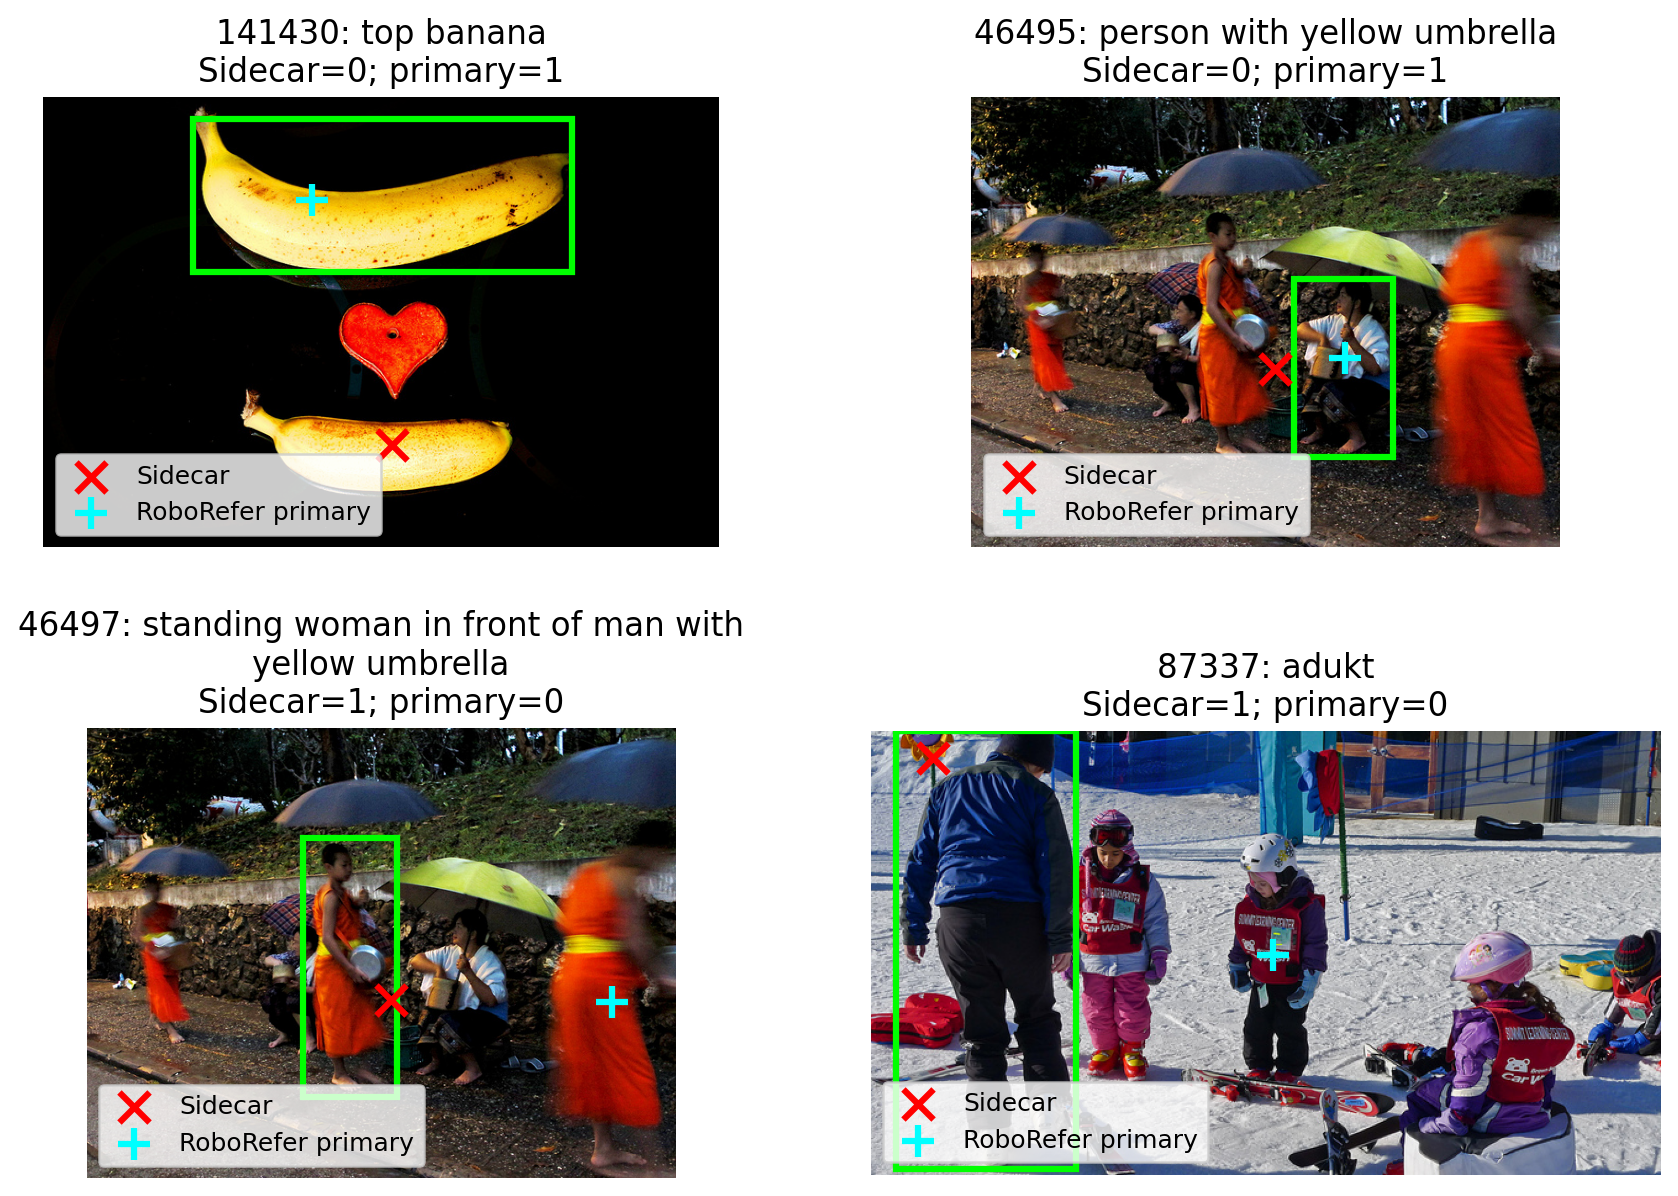
\includegraphics[width=0.98\linewidth,height=0.60\textheight,keepaspectratio]{figures/benchmark_20261007/refcoco_primary_cases_report.png}
\caption{RefCOCO: bbox GT xanh lá chỉ dùng hậu kiểm, điểm Sidecar đỏ, điểm
RoboRefer primary cyan. Hình gồm các ca sửa được và các ca làm sai khi đổi
nguồn target; không dùng ảnh minh họa tổng hợp hoặc chỉnh prediction.}
\label{fig:refcoco-cases}
\end{figure}

\noindent\small
Ở câu \texttt{top banana}, Sidecar chọn banana phía dưới trong khi primary
chỉ đúng banana phía trên. Case đã chạy lại từ RGB/depth bằng entry point
live: điểm primary $[254,109]$ trên ảnh $640\times480$, tương ứng $[254,97]$
trên ảnh gốc $640\times427$; Sidecar MAP vẫn ở $[330,370]$ trong hệ inference.
Đây là lỗi binding thuộc tính/vị trí, không chỉ lỗi nhận biết lớp banana.
Các case \texttt{standing woman in front of man with yellow umbrella} và
\texttt{adukt} ở hàng dưới cho thấy primary vẫn có thể sai dù Sidecar đúng.
Vì vậy giữ nguyên 7 ca bị làm sai trong thống kê paired, không chỉ trình bày
187 ca được sửa.
\end{landscape}

\begin{landscape}
\section{Case thật: các lỗi còn lại trên RefCOCO+}
\begin{figure}[H]\centering
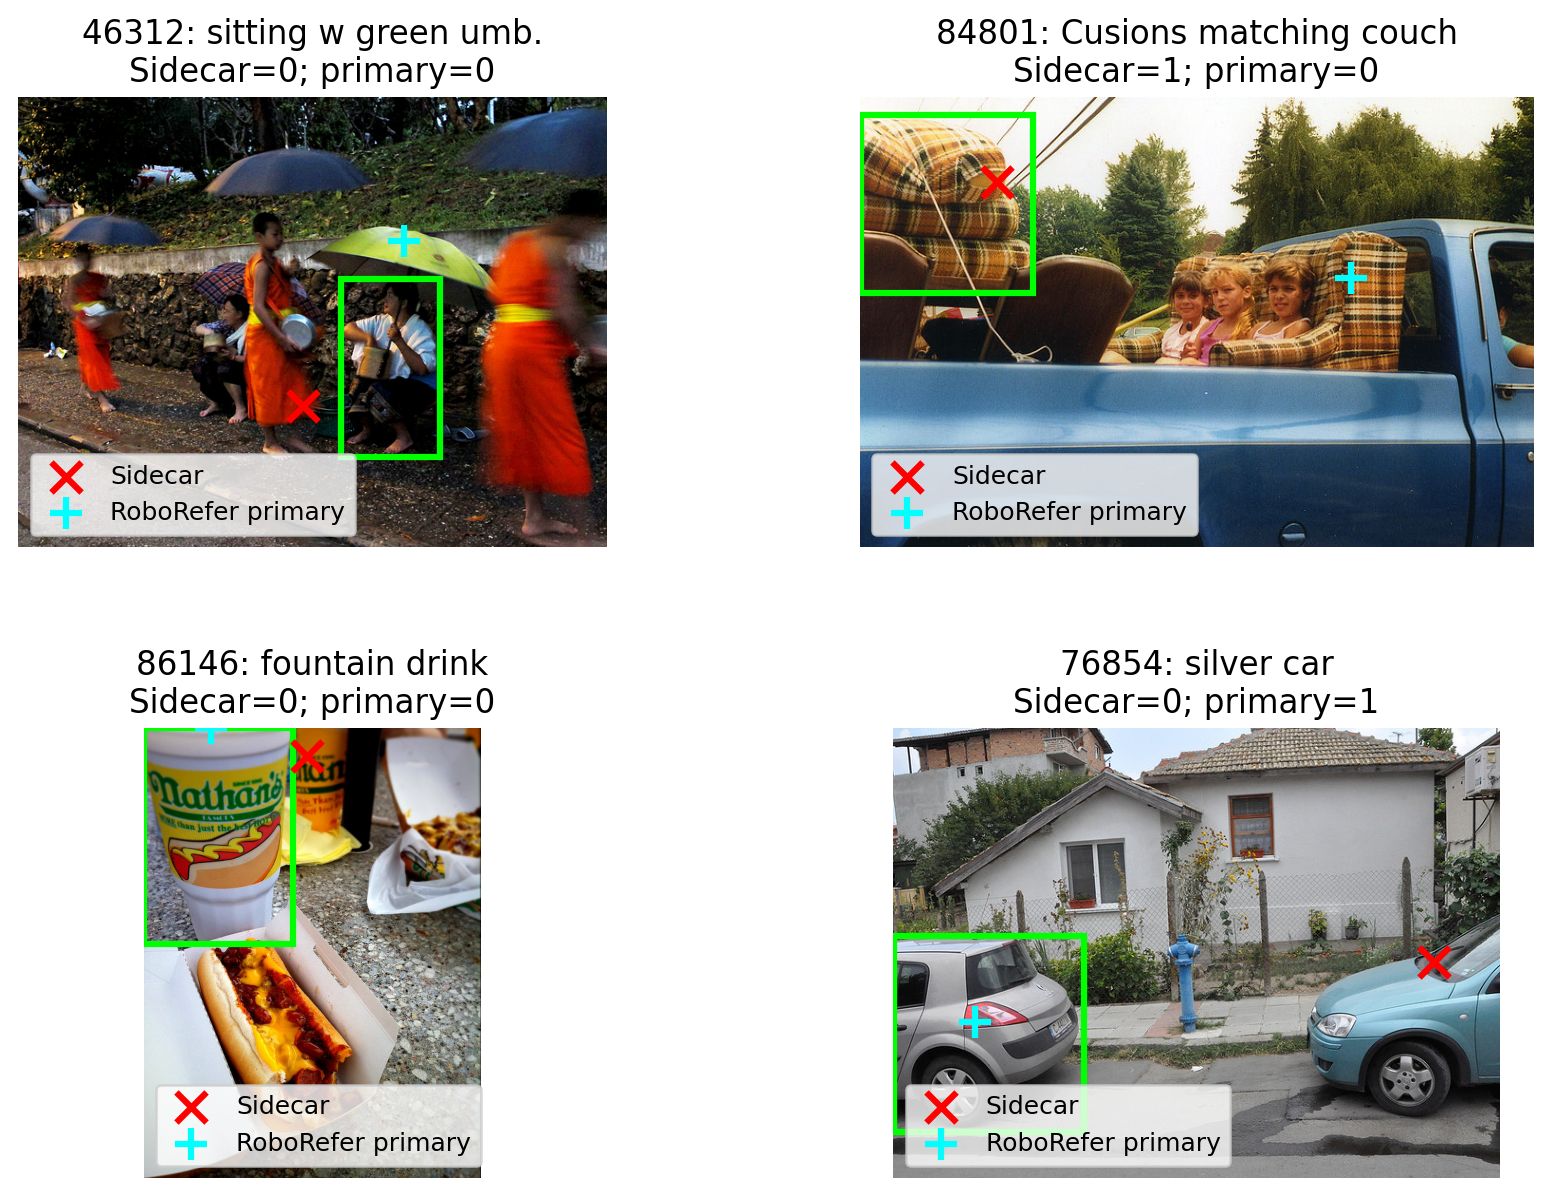
\includegraphics[width=0.98\linewidth,height=0.60\textheight,keepaspectratio]{figures/benchmark_20261007/refcoco_plus_cases_report.png}
\caption{RefCOCO+: ba case sai primary và một case được sửa khi đổi nguồn
target. Màu điểm/bbox như Hình~\ref{fig:refcoco-cases}.}
\label{fig:refcocoplus-cases}
\end{figure}

\noindent\small
\texttt{sitting w green umb.}: primary chọn ô xanh, trong khi target GT là
người ngồi dưới ô. \texttt{Cusions matching couch}: primary chọn đệm có
họa tiết tương tự ở bên kia, ngoài bbox GT; ghi nhận sai reference theo annotation.
\texttt{fountain drink}: điểm $[95,0]$ trong khi bbox bắt đầu ở $y=0,25$;
đây là lỗi sát biên theo metric, chưa là bằng chứng chọn sai loại vật.
Một ca khác, \texttt{HORSE IN THE SUN}, cách bbox 1,43 pixel. Không tăng
tolerance để loại hai ca này khỏi 27 lỗi. Case \texttt{silver car} cho thấy
primary tìm đúng xe bạc, còn Sidecar dồn điểm sang xe xanh trong cùng ảnh.
\end{landscape}

\section{Hướng cải tiến kiến trúc và thứ tự triển khai}
\subsection{Ưu tiên 1: giữ grounding RoboRefer làm đầu ra chính}
Hướng đã tích hợp là:
\begin{center}\small
RGB/depth + câu lệnh $\longrightarrow$ frozen RoboRefer đầy đủ
$\longrightarrow$ điểm target primary\\[0.3em]
features + câu lệnh $\longrightarrow$ Sidecar $\longrightarrow$ anchor/evidence\\[0.3em]
target primary + anchor $\longrightarrow$ parser/verifier
$\longrightarrow$ evidence $\longrightarrow$ calibrator mới.
\end{center}
Entry point \code{new/scripts/infer_roborefer_primary.py} và adapter
\code{new/src/pcrau/roborefer_primary.py} đã chạy được.
Primary giữ đúng một normalized point; điểm invalid/multiple/out-of-range
không fallback sang Sidecar hoặc tự clamp. Không tạo heatmap Gaussian/one-hot
từ point rồi gọi đó là predictive uncertainty.

Vai trò nghiên cứu của P-CRA-U chuyển sang kiểm chứng ràng buộc không gian
và hiệu chuẩn xác suất lỗi của prediction backbone. Target head Sidecar vẫn
có thể giữ để đối chiếu hoặc làm auxiliary head, nhưng không tự ghi đè
đường grounding đang cho kết quả tốt hơn trên hai pilot.

\subsection{Ưu tiên 2: tạo evidence và fit calibration cho đúng điểm primary}
Calibrator33/44/60 cũ nói về MAP Sidecar. Thay point trong JSON nhưng giữ
risk đó sẽ khiến vị trí và xác suất lỗi thuộc hai prediction khác nhau.
Cần freeze nhánh primary và schema mới, chạy train/dev để kiểm tra kỹ thuật,
rồi tạo evidence trên calibration đã tách. Event mục tiêu là
\[
E_{\rm primary}
= \{\mathrm{truth}\ne\mathrm{FOUND}\}
\ \lor\ \{\hat p_{\rm RoboRefer}\notin M_{\rm target}\}.
\]
Fit calibrator và chọn threshold chỉ trên calibration; sau đó reevaluate IID
cũ và báo lại grounding, coverage, selective risk, Brier/NLL/ECE của cùng
pipeline. Không fit hoặc chọn ngưỡng trên hai public pilot đã xem.
Trạng thái hiện tại của primary là risk/threshold chưa xác định;
valid point báo \texttt{REVIEW\_UNCALIBRATED}, chưa tự \texttt{EXECUTE}.

\subsection{Ưu tiên 3: gắn các đại lượng uncertainty với đúng biến dự đoán}
\begin{table}[H]\centering\small
\caption{Việc cần làm khi chuyển target cuối sang RoboRefer. Đây là kế hoạch,
không phải kết quả đã chứng minh trên benchmark.}
\begin{tabularx}{\linewidth}{P{2.8cm} Y}
\toprule
Thành phần & Điều chỉnh cần kiểm chứng\\
\midrule
Semantic & Lấy evidence tại target primary, mở rộng phrase matching khi có supervision; phân biệt identity lớp với chọn đúng instance.\\
Spatial & MC map Sidecar chỉ đo Sidecar. Muốn uncertainty của grounding RoboRefer cần cơ chế predictive distribution có căn cứ và đánh giá riêng.\\
Relation & Tính lại từ primary target và đúng anchor. Signed margin giữa hai điểm là evidence, chưa tự là xác suất đúng/sai quan hệ.\\
Depth & Lấy lại prediction tại vị trí primary; kiểm tra hệ đơn vị và dữ liệu reference. Pseudo-depth public không phải metric-depth GT.\\
Occlusion /\newline completion & Kiểm tra reference completion cho cùng vật/vị trí, đánh giá bằng labels phù hợp; không suy ra chất lượng amodal từ point-in-box.\\
\bottomrule
\end{tabularx}
\end{table}

MC Dropout có thể tiếp tục dùng ở các head phụ trợ có dropout được huấn luyện.
Các phân bố đó phải ghi rõ phạm vi, không gọi là bất định epistemic của toàn
bộ RoboRefer hoặc năm nguồn nhân quả đã phân rã. Một disagreement giữa điểm
Sidecar và RoboRefer là feature tiềm năng; cần fit/kiểm chứng trước khi gọi
nó là xác suất lỗi.

\subsection{Ưu tiên 4: cải tiến binding/verifier và kiểm chứng đóng góp}
Sau khi primary/calibration thống nhất, kiểm tra anchor binding trên train/dev,
gồm đổi vai target--anchor và anchor không hiện diện. Trong phạm vi trái/phải,
verifier dùng primary point với anchor prediction trong cùng hệ ảnh.
Mở rộng parser/quan hệ phải có annotation và evaluator phù hợp, không chỉ
thêm tên predicate. Ca unsupported cần được ghi rõ; nếu dùng fallback hoặc
hard veto, phải đánh giá ảnh hưởng coverage và risk thay vì mặc định an toàn.

Nếu cần nâng Sidecar chuyển miền, ưu tiên thử biểu diễn ngôn ngữ pretrained
hoặc phrase-conditioned features từ backbone và train/dev đa dạng hơn.
Đây là thay đổi cần controlled experiments, không thêm dữ liệu public val
đã chấm rồi báo lại như test độc lập. Thực hiện ablation giữ chung
checkpoint/split: primary, primary+verifier, primary+uncertainty và pipeline
đầy đủ, để tách đóng góp từng cơ chế.

\section{Kết luận}
Hai pilot công khai cho thấy target head Sidecar chưa chuyển miền tốt, trong
khi grounding đầy đủ của RoboRefer đạt 93,67\% trên RefCOCO và 91,00\% trên
RefCOCO+. Kết quả 6/100 trên RefSpatial cũng cho thấy hạn chế rõ của cấu hình
Sidecar khi gặp câu lệnh spatial referring phức tạp. Vì vậy, ưu tiên hiện tại
là giữ điểm RoboRefer, thống nhất evidence quanh điểm đó và hiệu chuẩn lại.

\begin{samepage}
Các số cao của primary là năng lực được kế thừa từ backbone. Phần đóng góp
của đồ án cần được chứng minh bằng binding, kiểm chứng quan hệ và chất lượng
quyết định chọn lọc, thay vì gán mức tăng grounding cho MC hoặc verifier khi
chưa có ablation. Chưa có đánh giá RefCOCOg/testA/testB, calibration primary
hoàn chỉnh hoặc kết quả robot motion từ các lượt benchmark này.
\par
\end{samepage}

\section*{Nguồn số liệu và cách biên dịch}
\addcontentsline{toc}{section}{Nguồn số liệu và cách biên dịch}
Số paper: Table 3 của arXiv:2506.04308v2; giữ nguyên 93.63 ở RefCOCOg test
của RoboRefer-2B-RFT như nguồn. Số đồ án lấy từ các artifacts đã lưu:
\begin{itemize}\small
\item \code{new/outputs/refcoco_val_pilot300_20261007/summary.json}
\item \code{new/outputs/pcrau_roborefer_primary_pilot300_20261007/summary.json}
\item \code{new/outputs/refcoco_plus_val_pilot300_20261007/summary.json}
\item \code{new/outputs/refcoco_plus_val_pilot300_20261007/error_audit.json}
\item \code{new/outputs/refspatial_location_frozen_20261007/summary.json}
\end{itemize}
Các đường artifact trên là provenance trong workspace, không là phụ thuộc
biên dịch. Ảnh gốc đã được đóng gói trong
\code{baocao1/figures/benchmark_20261007/}; hai figure bốn panel của báo cáo
được render lại từ đúng ảnh, GT bbox và prediction đã lưu, chỉ tăng độ rõ
của nhãn/marker, không sửa điểm. Nguồn và SHA256 nằm trong
\code{baocao1/benchmark_image_sources.json}. File này độc lập với báo cáo
\code{bao_cao_tien_do.tex} người dùng đã sửa.

Chạy XeLaTeX hai lần từ thư mục \code{baocao1}, hoặc chọn XeLaTeX trên
Overleaf và tải file này cùng thư mục \code{figures/benchmark_20261007/}.
Không cần BibTeX; tài liệu tham khảo nằm trong file nguồn.

\begin{thebibliography}{9}
\bibitem{roborefer}
E. Zhou và cộng sự.
\emph{RoboRefer: Towards Spatial Referring with Reasoning in Vision-Language
Models for Robotics}. arXiv:2506.04308v2, 2025, Table 3 và mục 4.3.
\url{https://arxiv.org/html/2506.04308v2#S4.T3}.

\bibitem{refer}
L. Yu và cộng sự. REFER: Referring Expression Datasets API, RefCOCO/+/g.
\url{https://github.com/lichengunc/refer}.
Mirror dùng trong thực nghiệm:
\url{https://huggingface.co/datasets/jxu124/refcoco-benchmark}.

\bibitem{refspatial}
BAAI. RefSpatial-Bench, Location split.
\url{https://huggingface.co/datasets/BAAI/RefSpatial-Bench}.

\bibitem{gal2016}
Y. Gal và Z. Ghahramani.
\emph{Dropout as a Bayesian Approximation: Representing Model Uncertainty
in Deep Learning}. ICML, PMLR 48:1050--1059, 2016.
\url{https://proceedings.mlr.press/v48/gal16.html}.
\end{thebibliography}
\end{document}
